\chapter{Konzeption}
\label{chapter-konzept}

In diesem Kapitel werden die zuvor erarbeiteten Erkenntnisse und Anforderungen genutzt, um konkrete
Funktionalitäten (\ref{section:funktionalitaeten}) zu definieren. Anschließend wird auf die
Systemarchitektur (\ref{section:architektur}) und Wahl der Frameworks (\ref{section:Frameworkwahl})
eingegangen.
\section{Funktionalität}
\label{section:funktionalitaeten}
Im Folgenden werden die für das System relevanten Funktionalitäten aufgeführt.
Jene beschreiben, wie das System die erarbeiteten Anforderungen erfüllt. Zur
besseren Lesbarkeit wurden die Funktionalitäten nach Nutzendengruppen aufgeteilt.

\subsection{Funktionalitäten für Ver- und Ausleihende}
Zu Beginn werden Funktionalitäten, welche für Verleihende und Ausleihende von
Bedeutung sind, näher erläutert (\ref{table:ft-b}).

\begin{table}[h]
    \centering
    \caption{Funktionalitäten für Ver- und Ausleihende}
    \begin{tabular}{lll}
        \arrayrulecolor{maincolor}\hline
        \sffamily\color{maincolor}ID & \sffamily\color{maincolor}Titel    &
        \sffamily\color{maincolor}Anforderungen
        \\
        \arrayrulecolor{maincolor}\hline
        Ft-VA-1                      & Authentifizierung über \ac{ldap}   &
        \anfref{F70} \anfref{F80}                                           \\
        Ft-VA-2                      & Übersicht über ausleihbaren Assets &
        \anfref{V20} \anfref{Z20} \anfref{F50} \anfref{K10} \anfref{F10}
        \anfref{F30}                                                        \\
        Ft-VA-3                      & Verfügbarkeit von Assets           &
        \anfref{V20} \anfref{Z20} \anfref{F50} \anfref{K10} \anfref{F10}
        \anfref{F30}                                                        \\
        Ft-VA-4                      & Zuständigkeitsbereich              &
        \anfref{F50}                                                        \\
        Ft-VA-5                      & Benachrichtigungen \& Erinnerungen &
        \anfref{F100} \anfref{F110} \anfref{F120}
        \\
        Ft-VA-6                      & Material-Suche                     &
        \anfref{V20} \anfref{Z20} \anfref{K10} \anfref{F10} \anfref{F30}
        \\
        Ft-VA-7                      & Filtern und Sortieren              &
        \anfref{V30} \anfref{F30} \anfref{F70}
        \\
        Ft-VA-8                      & Detailansicht                      &
        \anfref{V50} \anfref{Z30} \anfref{F40} \anfref{F50}
        \\
        \arrayrulecolor{maincolor}\hline
    \end{tabular}
    \label{table:ft-b}
\end{table}

{\sffamily\color{maincolor}{Ft-VA-1 | Authentifizierung über \ac{ldap}}}\\
Mithilfe der Verknüpfung zum \ac{ldap}-System des \ac{imis}, können sich Nutzende mit einem bereits
existierenden IDM Account einloggen \cite{howes_x500_1993}. Folglich muss kein neues Konto erstellt
werden. Außerdem kann überprüft werden, ob es sich bei der Anmeldung um Studierenden oder \ac{wimi}
handelt, um entsprechende Systemrechte zu vergeben. Des Weiteren verhindert die Nutzung des
\ac{ldap}-Systems das Eindringen unbefugter Personen.


    {\sffamily\color{maincolor}{Ft-VA-2 | Übersicht über ausleihbare Assets }}\\
Die Übersicht, der am \ac{imis} vorhandenen Assets wurde mittels Kategorien
umgesetzt, welche aus \textit{Snipe-IT} abgeleitet werden konnten. Dafür gibt es
eine Übersicht, bei der alle Assets eingesehen werden können. Die einzelnen
Kategorien beinhalten Unterkategorien. In der Übersicht werden Informationen wie
Name, Seriennummer, Marke und Status eines Assets angezeigt.

    {\sffamily\color{maincolor}{Ft-VA-3 |  Verfügbarkeit von Assets }}\\
Der Status eines Asset (ausleihbar und herausgegeben) muss klar ersichtlich sein. Dies geschieht
mittels Farbcodierung. Durch Die Farbcodierung können Nutzende schneller relevante Informationen
filtern, was insbesondere für den Status eines Assets wichtig ist.


    {\sffamily\color{maincolor}{Ft-VA-4 | Zuständigkeitsbereich }}\\
Um für Ausleihende Kontaktinformationen anzeigen zu können \textit{(Ft-A-6)},
müssen die Zuständigkeitsbereiche eingetragen werden können. Außerdem sollten
alternative Ansprechpartner:innen kenntlich gemacht werden, um Abholtermine
aufgrund von Krankheit oder Homeoffice nicht verschieben zu müssen. Für
Rückfragen zu einem Asset sind Kontaktinformation zu Ansprechpartner:innen
(Verleihende) sowie E-Mail-Adressen hinterlegt.

    {\sffamily\color{maincolor}{Ft-VA-5 | Benachrichtigungen \& Erinnerungen
        }}\\
Verleihende werden nach dem Ausleihen eines von ihnen verantwortlichen Assets benachrichtigt. Die
Benachrichtigung umfasst, wer das Asset wann reserviert hat und wann die Abholung für das Asset
stattfinden soll. Außerdem wird es eine direkte Weiterleitungsmöglichkeit geben, sollten Verleihende
verhindert sein. Nachdem die Reservierung eines Assets stattgefunden hat, erhalten Ausleihende eine
Zusammenfassung über die Ausleihdaten und einen Hinweis, wann die Abholung stattfindet. Außerdem
werden Kontaktinformation des Verleihenden angezeigt (Name, E-Mail und Lagerort des Assets).
Zusätzlich erhalten Verleihende und Ausleihende eine Erinnerung, sobald die Abholung oder Rückgabe
eines Assets ansteht.

    {\sffamily\color{maincolor}{Ft-VA-6 | Material-Suche }}\\
Die Material-Suche umfasst eine Einteilung der Assets nach Kategorie, sowie die gezielte Suche nach
der Verfügbarkeit der Assets (ausleihbar und herausgegeben). Das gezielte Suchen nach Verfügbarkeit
wird durch die Aufforderung, den Ausleihzeitraum anzugeben, ermöglicht. Daraufhin gibt es die
Möglichkeit gewünschte Materialien in einem Suchfeld einzugeben oder über die Kategorien nach dem
Asset zu suchen. Die Vorschläge umfassen Assets oder Kategorien.

    {\sffamily\color{maincolor}{Ft-VA-7 | Filtern und Sortieren }}\\
Um das Finden der Assets leichter zu gestalten, sollen Nutzende stets nach Kategorie, Nutzen und
Verfügbarkeit filtern können. Um bei der Anzeige einen Überblick über die Menge der Assets behalten
zu können, wird die Anzahl der Assets in der ausgewählten Kategorie angezeigt.

    {\sffamily\color{maincolor}{Ft-VA-8 | Detailansicht }}\\
In der Detailansicht werden die Assets und deren Eigenschaften dargestellt. Hierbei werden
Informationen wie Name, Artikelbeschreibung, technische Details und Kontaktinformation der
Verleihenden dargestellt. Des Weiteren kann der Ausleihzeitraum eingestellt und die Zeiträume der
Verfügbarkeit eines Assets eingesehen werden. In Form eines Buttons wird sichtbar, dass das Asset
zur Ausleihe hinzugefügt werden kann.


\subsection{Funktionalitäten für Verleihende}
Im Folgenden werden Funktionalitäten, welche für Verleihende von Bedeutung sind
näher erläutert (\ref{table:ft-v}).

\begin{table}[h]
    \centering
    \caption{Funktionalitäten für Verleihenden }
    \begin{tabular}{lll}
        \arrayrulecolor{maincolor}\hline
        \sffamily\color{maincolor}ID & \sffamily\color{maincolor}Titel  &
        \sffamily\color{maincolor}Anforderungen
        \\
        \arrayrulecolor{maincolor}\hline
        Ft-V-1                       & Verwaltungsansicht               & \anfref{F60}
        \\
        Ft-V-2                       & Bearbeiten des Assetstatus       & \anfref{F150} \\
        Ft-V-3                       & Kalenderansicht  für Verleihende &
        \anfref{V50} \anfref{Z30} \anfref{F40} \anfref{F50}
        \\
        Ft-V-4                       & Pflege von Assets                &
        \anfref{F130}                                                                   \\
        Ft-V-5                       & Pflege der Datenbank             &
        \anfref{F140}                                                                   \\
        \arrayrulecolor{maincolor}\hline
    \end{tabular}
    \label{table:ft-v}
\end{table}

{\sffamily\color{maincolor}{Ft-V-1 | Verwaltungsansicht }}\\
Die Verwaltungsansicht umfasst eine Aufgabenliste mit zwei Tabs. Die Tabs umfassen Abholungs- oder
Rückgabetermine. Über eine Kalenderübersicht können die Abholungs- oder Rückgabetermine der
einzelnen Tage eingesehen werden.

    {\sffamily\color{maincolor}{Ft-V-2 | Bearbeiten des Assetstatus }}\\
Assets, welche an Ausleihende übergeben wurden, müssen zunächst manuell in ihrem
Status bestätigt werden. Hierfür ist eine simple Button-Funktion vorgesehen,
sodass der Status des Assets schnell aktuell gehalten werden kann. Außerdem soll
das System, nachdem eine Abholung oder Rückgabe stattgefunden hat, eine
Benachrichtigung an Verleihende senden, sollte der Status nicht bereits
bestätigt worden sein.

    {\sffamily\color{maincolor}{Ft-V-3 | Kalenderansicht für Verleihende}}\\
Die Kalenderansicht für Verleihende beinhaltet eine Übersicht über alle Assets,
welche in diesem Moment verliehen sind. Mithilfe einer Monatsübersicht werden
Termine zur Asset-Abholung, Rückgabe oder zur Wartung angezeigt.


    {\sffamily\color{maincolor}{Ft-V-4 | Pflege von Assets   }}\\
Mithilfe des Zuständigkeitsbereichs \textit{(Ft-V-2)} kann die Pflege der Assets
besser kontrolliert werden. Außerdem können durch Erinnerungen und Checkliste
Wartungen weniger leicht vergessen werden und besser aufgeteilt werden.

    {\sffamily\color{maincolor}{Ft-V-5 | Pflege der Datenbank }}\\
Das einpflegen der Assets ist die Grundvoraussetzung für die Nutzung des Reservieurngstools. Diese
Funktionalität wird bereits durch Snipe-IT bereitgestellt. Aufgrund der Vollständigkeit wird diese
Funktionalität ebenfalls mit aufgeführt.

\subsection{Funktionalitäten für Ausleihende}
Im Folgenden werden Funktionalitäten, welche für Ausleihende von Bedeutung sind,
näher erläutert (\ref{table:ft-A}).

\begin{table}[h]
    \centering
    \caption{Funktionalitäten für Ausleihende }
    \begin{tabular}{lll}
        \arrayrulecolor{maincolor}\hline
        \sffamily\color{maincolor}ID & \sffamily\color{maincolor}Titel &
        \sffamily\color{maincolor}Anforderungen
        \\
        \arrayrulecolor{maincolor}\hline
        Ft-A-1                       & Dashboard                       &
        \anfref{F60}                                                     \\
        Ft-A-2                       & Reservierungs-Checkout          &
        \anfref{F60} \anfref{F150}                                       \\
        Ft-A-3                       & Kalenderansicht für Ausleihende &
        \anfref{V50} \anfref{Z30} \anfref{F40} \anfref{F50}
        \\
        \arrayrulecolor{maincolor}\hline
    \end{tabular}
    \label{table:ft-A}
\end{table}


{\sffamily\color{maincolor}{Ft-A-1 | Dashboard }}\\
Das Dashboard soll Ausleihenden helfen, einen Überblick zu erlangen. Für
Erstnutzende sind Hinweise für die Material-Suche in Form von Buttons gegeben.
Für Ausleihende, welche bereits Assets ausgeliehen haben, wird eine Übersicht über
laufende, kommende und vergangene Reservierungen angezeigt. Wichtige
Informationen, wie der Zeitraum, werden direkt auf einen Blick ersichtlich.

    {\sffamily\color{maincolor}{Ft-A-2 | Reservierungs-Checkout }}\\
Mithilfe des Reservierungs-Checkouts können alle ausgewählten Assets überblickt werden. Außerdem
werden alle Ausleihdaten, wie Zeitraum der Ausleihe, Abholung und Rückgabe aufgeführt. Des Weiteren
gibt es die Möglichkeit alle Ausleihdaten bearbeiten zu können, sollte ein Datum oder eine Uhrzeit
unpassend sein. Nach Bestätigung einer Reservierung gilt die Reservierung des Assets als
abgeschlossen.

    {\sffamily\color{maincolor}{Ft-A-3 | Kalenderansicht für Ausleihende}}\\
Die Kalenderansicht für Ausleihende beinhaltet eine Übersicht, über die Verfügbarkeit eines
einzelnen Assets. Diese wird angezeigt, sobald sich Nutzende auf der Detailsansicht eines Assets
befinden und den Ausleihzeitraum angeben. Außerdem befindet sich eine Kalenderübersicht in der
Suche, welche über das Hamburger-Menü erreichbar ist, um nach dem gewünschten Ausleihzeitraum zu
suchen.


\section{Systemarchitektur}
\label{section:architektur}
Die Systemarchitektur gibt eine Übersicht über die technische Umsetzung des
Systems und bildet die Basis der Realisierung von Software-Systemen
\cite{dumke_software-metriken_2000}. Diese besteht im Wesentlichen aus den
folgenden drei Komponenten: dem \textit{Snipe-IT Server}, dem
\textit{Reservierungsinterface} und dem \textit{Frontend}.

Aufbauend auf den Anforderungen und der am \ac{imis} bereits eingesetzten Asset Managementsoftware
\textit{Snipe-IT} werden im Folgenden die gewählten Frameworks erläutert. Um ein besseres
Verständnis für die Architektur des entwickelten Software-Systemes voraussetzen zu können, wird nach
dem C4-Modell zur Visualisierung von Softwarearchitektur der Aufbau der Architektur mit den
Teilkomponenten detaillierter dargestellt \cite{brown2013software}.

\subsection{Voraussetzungen für die Frameworkwahl}
\label{section:Frameworkwahl}
Die Frameworkwahl nimmt durch die unterschiedlichen Arbeitsweisen und Funktionen
der Frameworks enormen Einfluss auf den Entwurf eines Systems und wird daher im
Folgenden näher erläutert.

Die Grundlage der Auswahl der im Rahmen dieser Arbeit eingesetzten Frameworks bilden die eingangs
beschriebenen Anforderungen (\ref{section:anforderung}). Dem System wird vorausgesetzt, dass es sich
um eine Web-Anwendung mit Fokus auf den Einsatz im mobilen Kontext (\anfref{R10}\anfref{R40})
handelt. Für Nutzende ist es wichtig, dass das System dauerhaft erreichbar ist (\anfref{R50}). Aus
funktionaler Sicht müssen die Frameworks eine Unterstützung für progressive Web-Applikationen
bieten. Folglich ist auch eine Unterstützung für HTTPS notwendig (\anfref{Q50}). Außerdem sollte es
einfache Möglichkeiten zur Verknüpfung von \ac{ldap} bieten (\anfref{K10} \anfref{F90}). Die konkrete
Wahl der Frameworks wird in \ref{subsec:level2} aufgeführt.

\subsection{C4-Modell zur Visualisierung von Softwarearchitektur}
Das Modell unterteilt die Architektur in vier Abstraktionsebenen (Level):
\textbf{Context}, \textbf{Container}, \textbf{Components} und \textbf{Code}.
Wobei im folgenden ausschließlich auf die ersten drei Ebenen eingegangen wird.
Des Weiteren werden die Bestandteile des Systems in vier Kategorien gegliedert:

\begin{itemize}
    \item \textbf{Person}: Stellt Nutzende eines Software-Systems dar.
    \item \textbf{Software-System}: Stellt die höchste Abstraktionsebene der
          Software dar.
    \item \textbf{Container}: Stellt einzeln ausführbare Teilkomponenten des
          Software Systems dar.
    \item \textbf{Component}: Stellt z.B. die Datenbank oder Anwendung dar.
\end{itemize}

{\sffamily\color{maincolor}{Level 1: Context}}

Das erste Level der Architekturvisualisierung nach dem C4-Modell, stellt die
entwickelte Software mithilfe eines Systemkontextdiagramms dar. \ref{fig:level1}
zeigt die Komponente des im Rahmen der Arbeit entwickelten Systems im
Zusammenhang mit der Asset-Managementsoftware \textit{Snipe-IT}.

\begin{figure}[h]
    \centering
    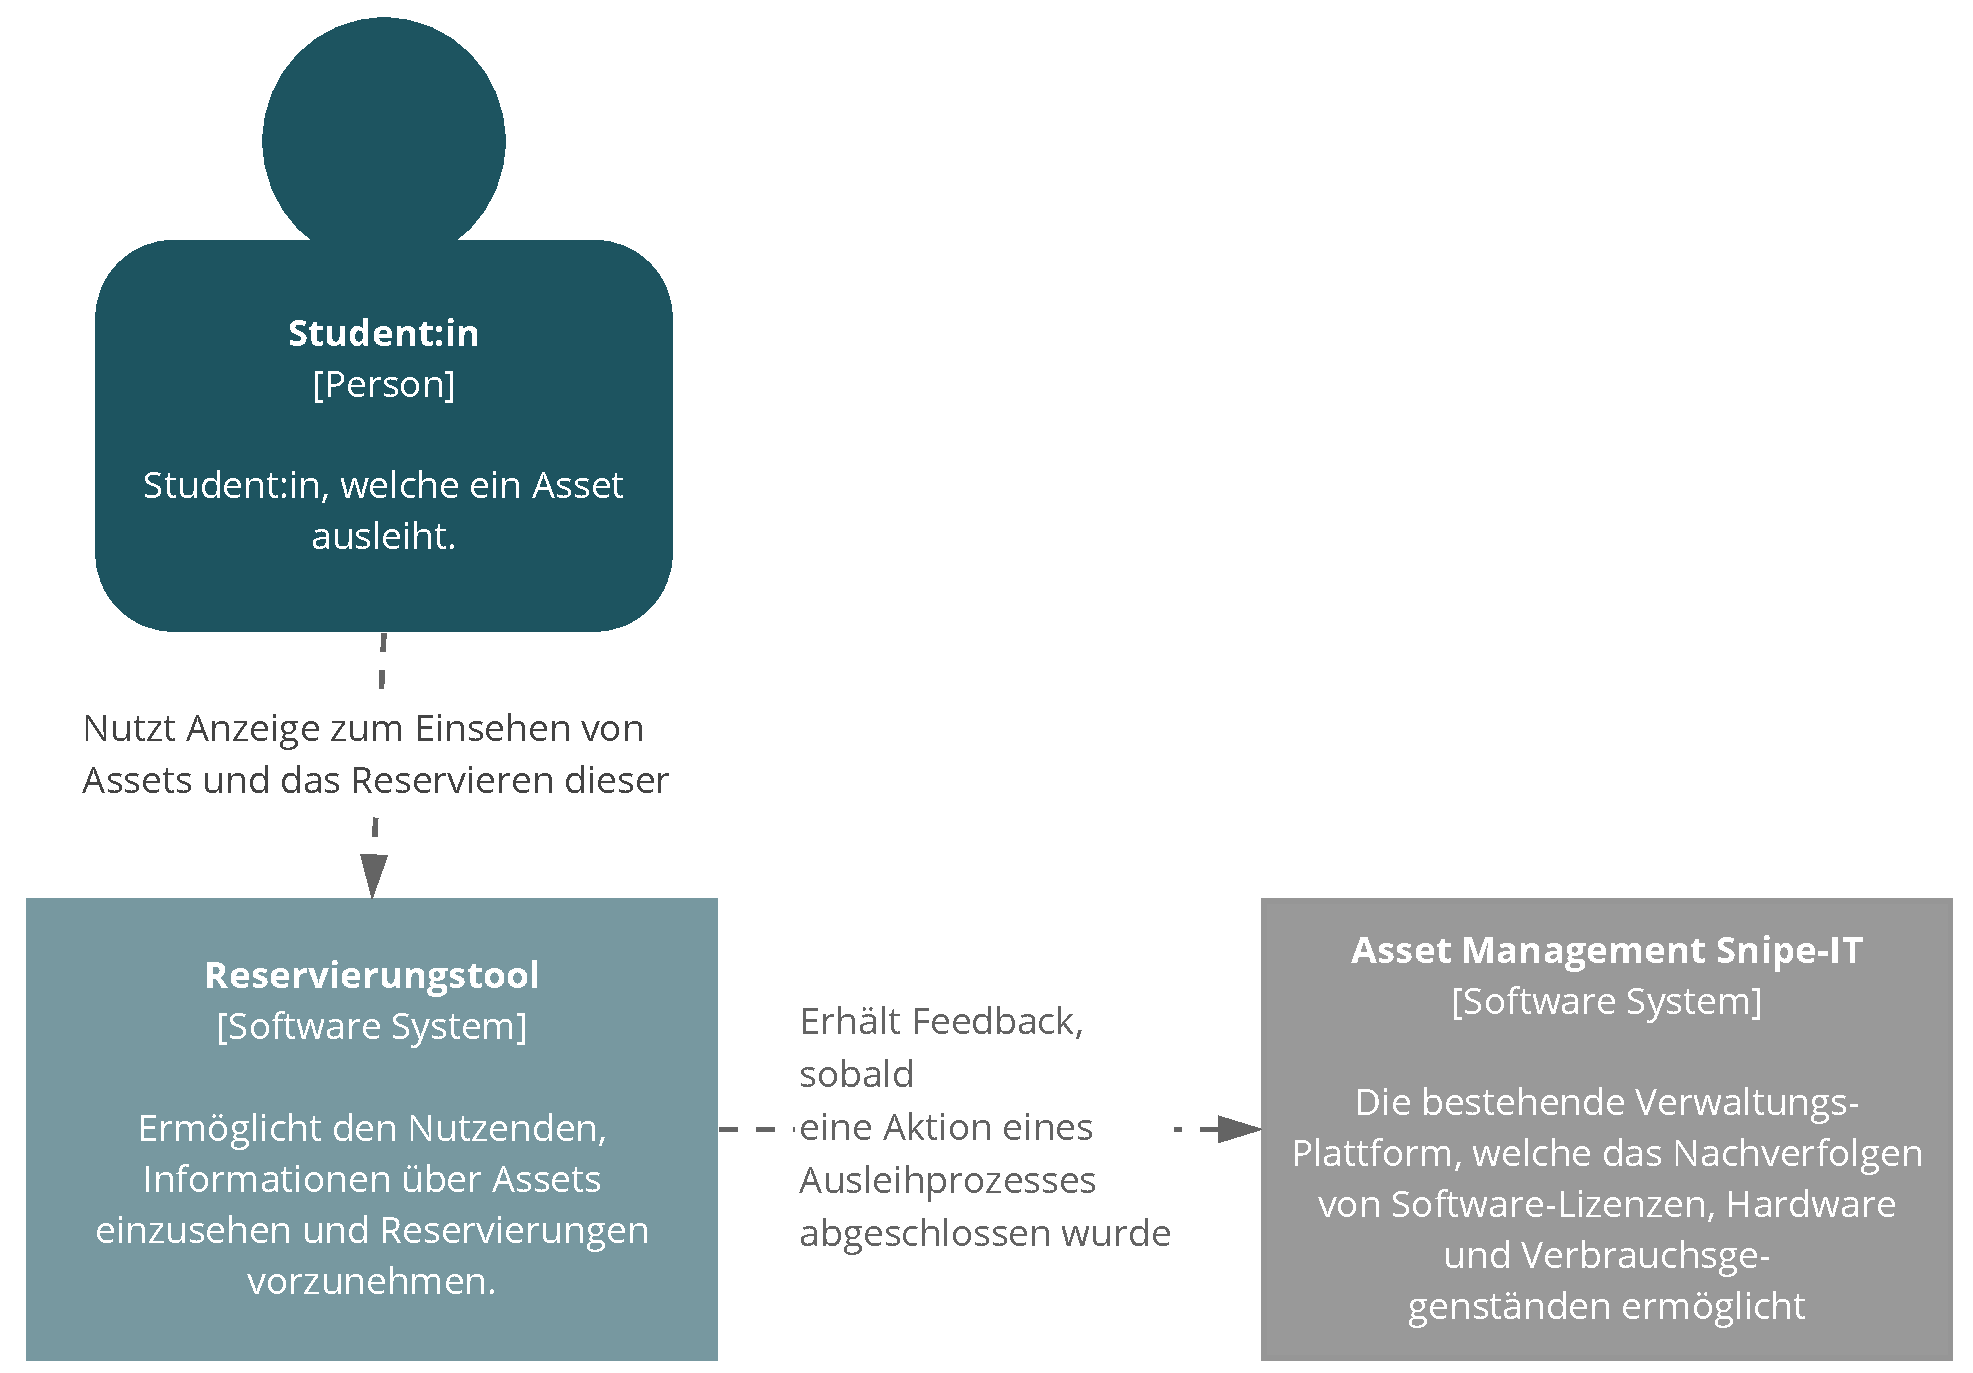
\includegraphics[scale=0.4]{Bilder/C4_1.pdf}
    \caption[C4-Modell Level 1: Context]{C4-Modell Level 1: Context nach
        \citeA{brown2013software}}
    \label{fig:level1}
\end{figure}

Der Kontext umfasst zwei Software-Systeme: das Reservierungstool und die Asset-Managementsoftware
\textit{Snipe-IT}. Das Reservierungstool bildet die Oberfläche für Ausleihende und ermöglicht es, die Assets
einzusehen, zu suchen und zu buchen. Außerdem laufen über die Web-Oberfläche alle administrativen
Aufgaben für Verleihende, wie das Aktualisieren eines Asset-Status. Hierzu nutzt die Web-App das
Reservierungsinterface, um auf die \textit{Snipe-IT} Funktionalitäten zuzugreifen.

\todo{Referenzierungen hinzufügen}
Die Basis für das in dieser Arbeit umgesetzte System schafft die Asset-Managementsoftware
\textit{Snipe-IT} \cite{noauthor_home_nodate}, welche bereits am \ac{imis} eingesetzt wird.
\textit{Snipe-IT} ist eine kostenlose, quelloffene IT-Asset-Verwaltungs-Plattform, welche das
Nachverfolgen von Software-Lizenzen, Hardware und Verbrauchsgegenständen ermöglicht. Genannte Assets
können über ein Dashboard hinzugefügt, verwaltet und gelöscht werden. Über Labels können Assets für
die Übersichtlichkeit in verschiedene Kategorien eingeordnet werden, während Tags ein Asset
eindeutig identifizieren (z. B. Seriennummer). Zudem ermöglicht das „Checkin/Checkout“-System die
Nachverfolgung aller Assets, falls diese zum Beispiel an Personen ausgeliehen werden. Zu jedem
Zeitpunkt kann ein Asset maximal einer Person zugeordnet werden, wodurch das mehrfache oder
gleichzeitige Ausleihen eines Assets verhindert wird. Darüber hinaus beschreiben Status-Label den
Zustands eines Assets und ob dieses ausgeliehen werden kann. Alle Funktionalitäten können zudem über
eine REST-API programmatisch genutzt werden. Des Weiteren verfügt \textit{Snipe-IT} über eine
Schnittstelle, welche die Integration von \ac{ldap} stark vereinfacht.

    {\sffamily\color{maincolor}{Level 2: Container}}
\label{subsec:level2}
Im zweiten Level werden die Container des Software-Systems gezeigt. Hierbei
werden Verantwortlichkeiten und die Kommunikation zwischen den Bestandteilen des
Software-Systems dargestellt (\ref{fig:level2})(Brown, 2021).

\begin{figure}[h]
    \centering
    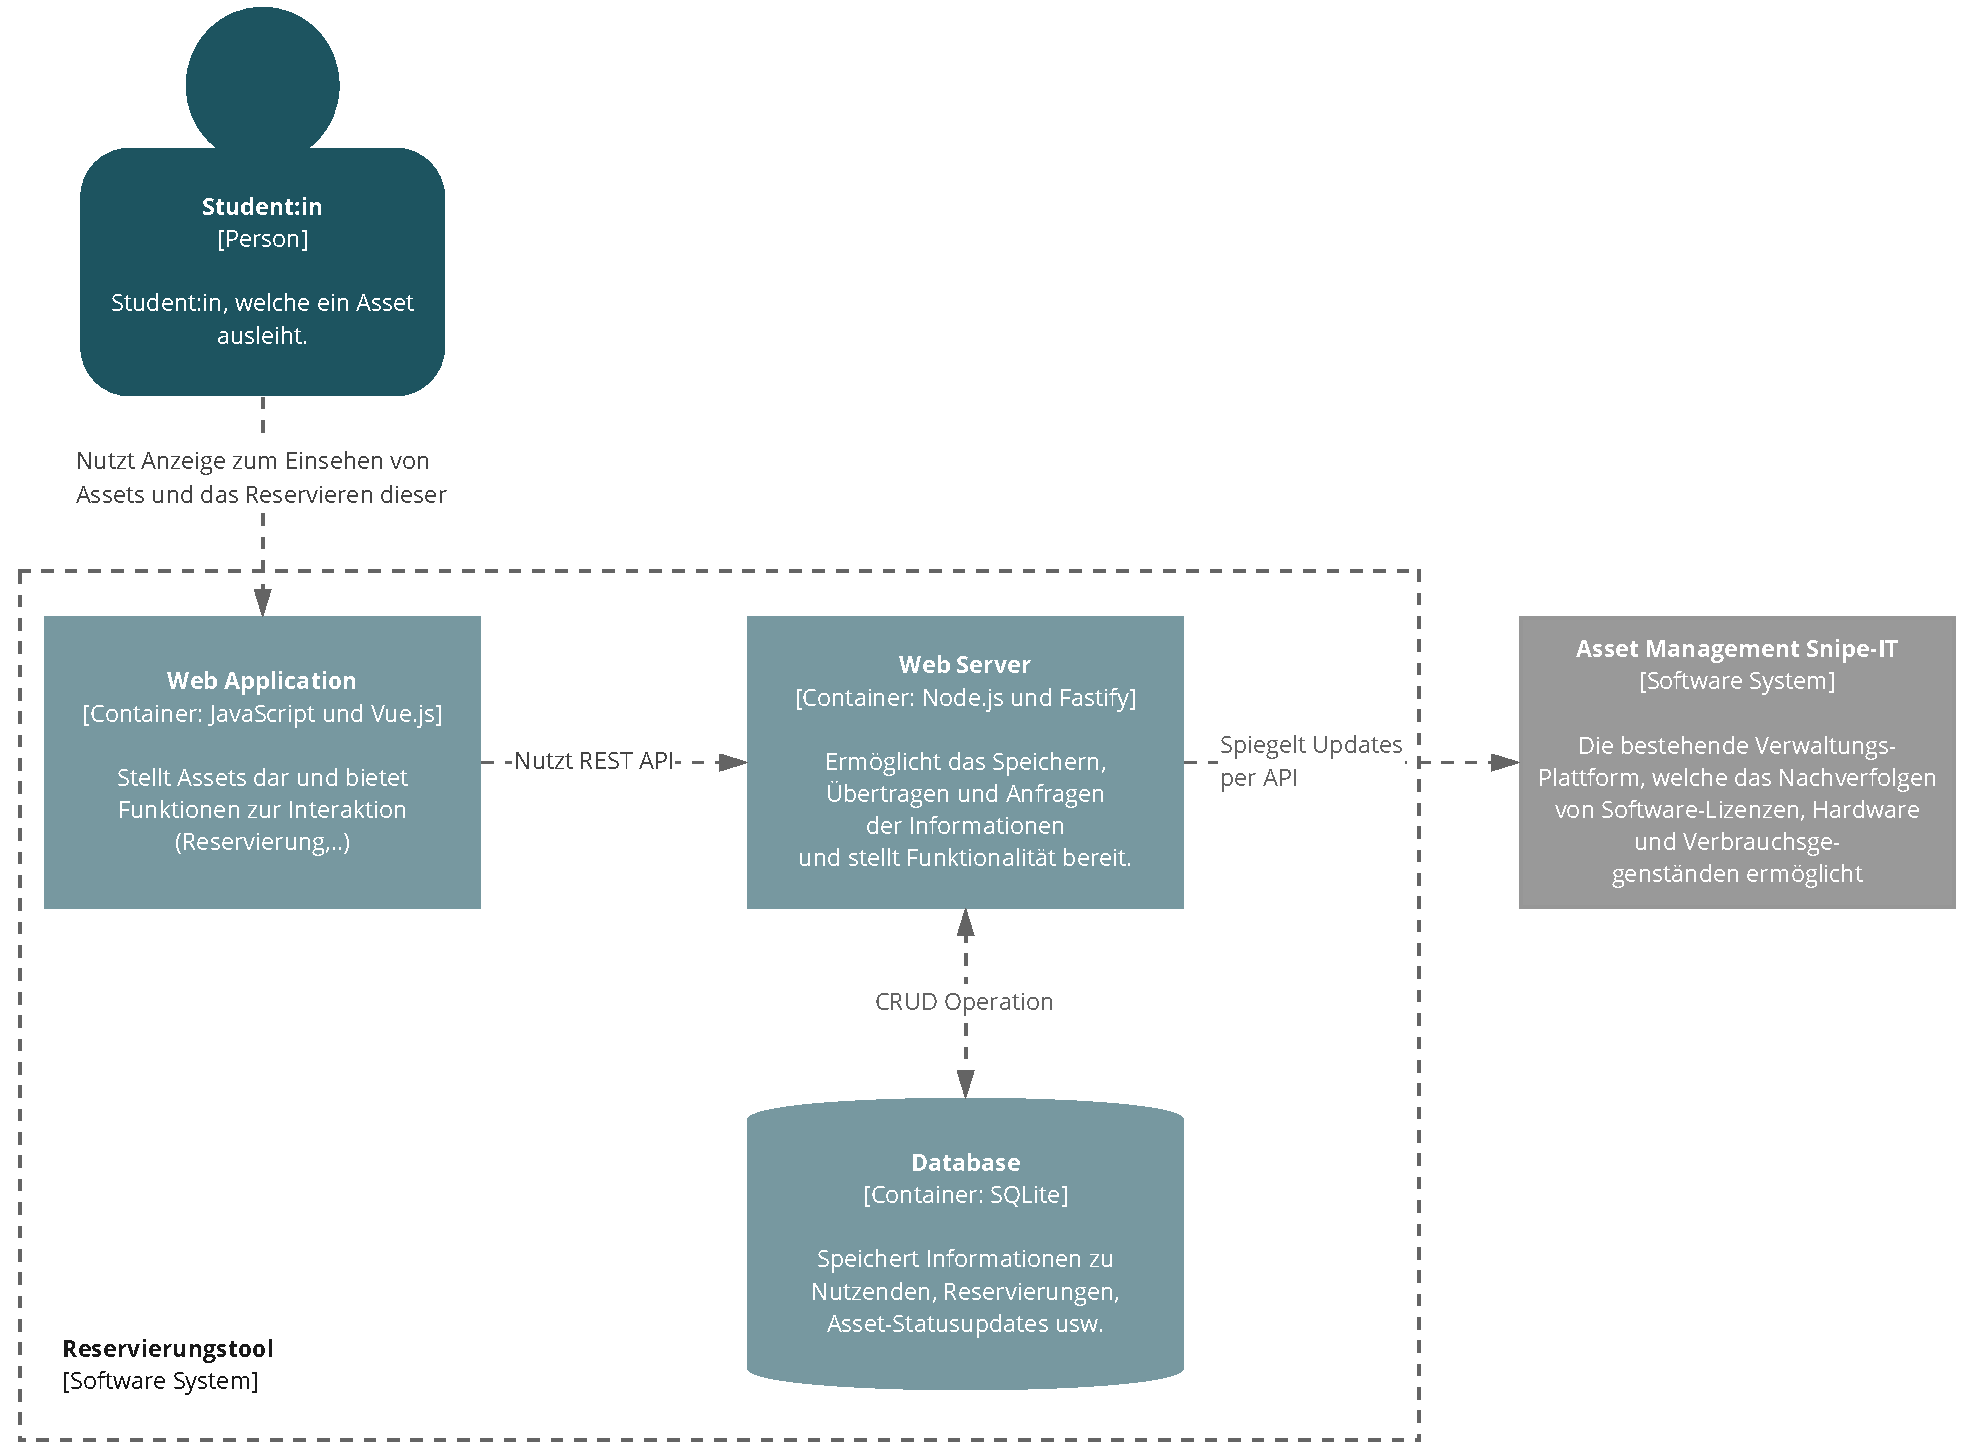
\includegraphics[scale=0.47]{Bilder/C4_2.pdf}
    \caption[C4-Modell Level 2: Container]{C4-Modell Level 2: Container nach
        \citeA{brown2013software}}
    \label{fig:level2}
\end{figure}

Für die Grundlage des Frontends wird Vue.js\footnote{\url{https://vuejs.org/}} verwendet. Vue.js ist
ein progressiver JavaScript Framework. Durch das Vite\footnote{\url{https://vitejs.dev/}}
Plugin-System kann eine PWA-Funktionalität mithilfe des
\inlinecode{vite-plugin-pwa}-Plugins\footnote{\url{https://github.com/vite-pwa/vite-plugin-pwa}}
schnell eingebunden werden. Zusätzlich wird Vue.js aufgrund der begrenzten Implementierungszeit und
bestehenden Erfahrung gewählt.

Das Reservierungsinterface nutzt die von Snipe-IT bereitgestellten Daten. Die
Hauptaufgabe der Schnittstelle ist das Reservieren von Assets in die Zukunft. Da
Snipe-IT selbst die zukünftige Reservierung nicht unterstützt, werden diese
Reservierungen stattdessen im Reservierungsinterface gespeichert. Die gesamte
Kommunikation zwischen Frontend und Snipe-IT wird somit über das
Reservierungsinterface stattfinden, um auch alle zukünftigen Reservierungen zu
berücksichtigen. Die Datenbank und API von Snipe-IT bilden die Ausgangsposition
des Systems. Folglich wird die Verwaltung und Speicherung der vorhandenen Assets
über Snipe-IT direkt abgewickelt. Über die bereitgestellte API werden die
gespeicherten Daten für alle weiteren Komponenten zur Verfügung gestellt.

    {\sffamily\color{maincolor}{Level 3: Components}}

Das dritte Level stellt die Container aus Level 2 genauer dar, um die
elementaren, strukturellen Bestandteile und Wechselwirkungen zwischen diesen
aufzuzeigen (Brown, 2021). Im Folgenden werden die Container
\textit{Web-Application} und \textit{Web Server} genauer betrachtet
(\ref{fig:level3}).

\begin{figure}[h]
    \centering
    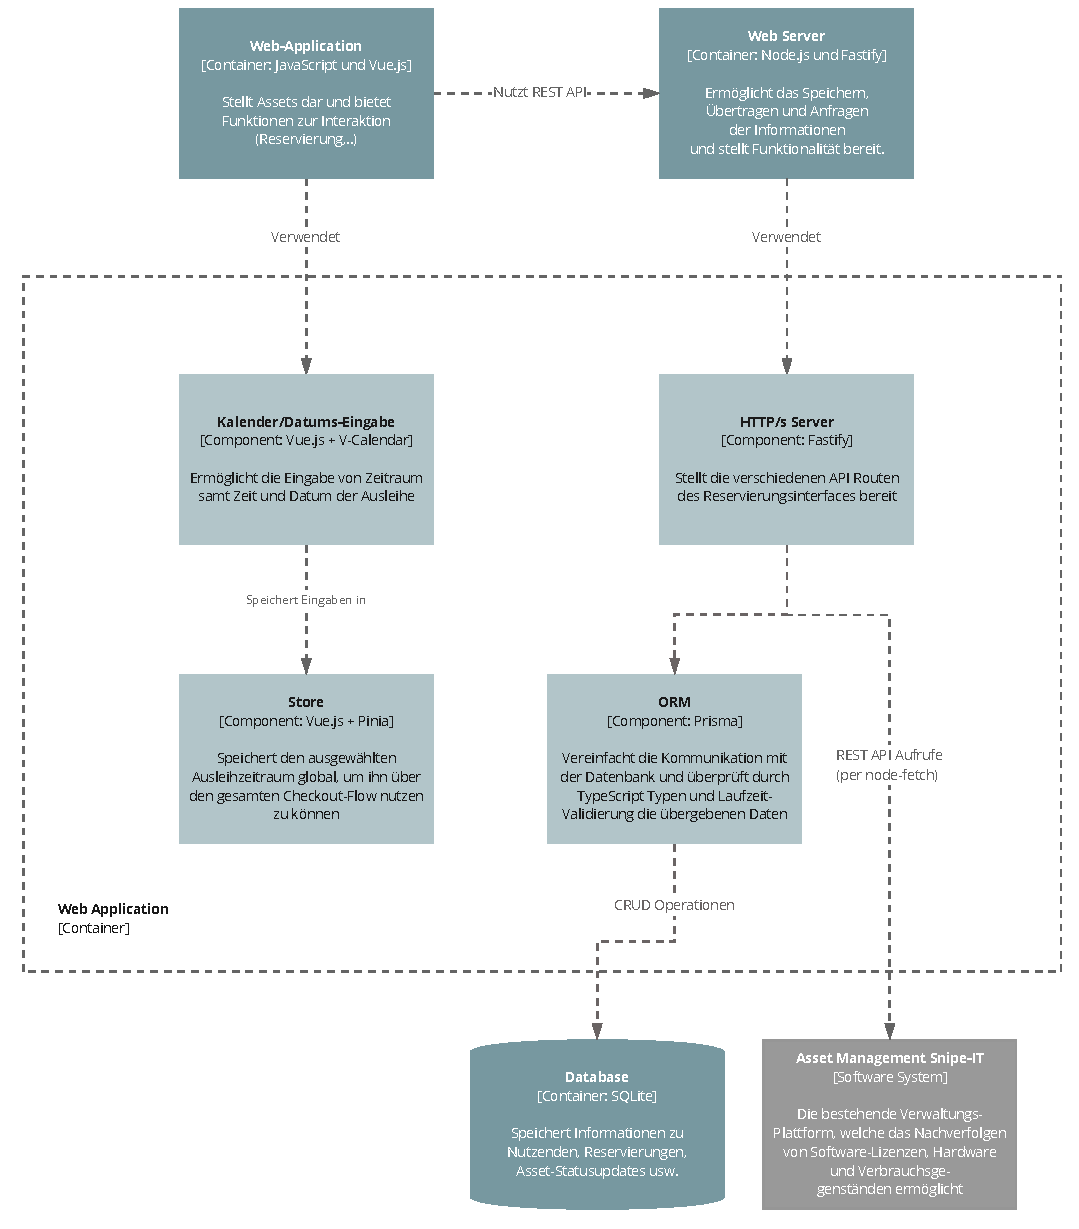
\includegraphics[scale=0.9]{Bilder/C4_3.pdf}
    \caption[C4-Modell Level 3: Components]{C4-Modell Level 3: Components nach \citeA{brown2013software}}
    \label{fig:level3}
\end{figure}

Die Web-Application nutzt die Kalenderkomponente
\textit{V-Calendar}\footnote{\url{https://vcalendar.io/layouts.html}}, welche die Eingabe von
Zeiträume und Uhrzeiten für das Ausleihen der Assets ermöglicht. Durch die umfangreiche API der
Komponente ist diese leicht anpassbar und erweiterbar. Die gewählten Zeiträume werden in einem
\textit{Pinia}-Store gespeichert, um sie komponenten-übergreifend nutzen zu können. Mithilfe des
\textit{Pinia}-Plugins
\textit{pinia-plugin-persistedstate}\footnote{\url{https://github.com/prazdevs/pinia-plugin-persistedstate}}
bleiben die Daten zudem auch beim Neuladen der Webapp erhalten.



Für das Reservierungsinterface wird ein Serverframework und eine
Speichermöglichkeit in Form einer Datenbank benötigt. Aufgrund der ausgeprägten
Pluginauswahl\footnote{\url{https://www.fastify.io/ecosystem/}} und breiten
Nutzung\footnote{\url{https://www.fastify.io/organisations/}} wird
\textit{Fastify}\footnote{\url{https://www.fastify.io/}} als Serverframework eingesetzt.
Als relationale Datenbank wird die quelloffene Software
\textit{SQLite}\footnote{\url{https://www.sqlite.org/index.html}} eingesetzt, da diese
zur Verwendung keine komplexe Einrichtung benötigt. Im Gegensatz zu Datenbanken
wie \textit{PostgreSQL} oder \textit{MySQL} benötigt SQLite keine Installation
eines Datenbank-Servers. Alle Daten werden in einer alleinstehenden Datei
gespeichert (https://www.sqlite.org/different.html). Trotz der simplen
Einrichtung bietet SQLite ein umfangreiches Sortiment an SQL-Funktionen und
unterstützt auch den Umgang mit großen Datensätzen
(https://www.sqlite.org/limits.html). Um den Zugriff und die Verwaltung der
Daten zu vereinfachen, wird zudem die ORM-Bibliothek
Prisma\footnote{\url{https://www.prisma.de/}} verwendet.

